\clearpage
\section{Benchmark-Konzept Mesh Netzwerke}\label{sec:BenchmarkKonzeptMeshNetzwerke}
\todo[inline]{Cyrill}

\subsection{Konzeptschema}\label{subsec:KonzeptschemaMesh}
\todo[inline]{Erläuterung des Konzeptschemas}

Für den Vergleich der 3 Mesh Netzwerkstacks Bluetooth Mesh (BT Mesh), Thread und Zigbee wird ein vom Mesh Protokoll unabhängiges Testkonzept umgesetzt welches in der Abbildung \ref{fig:MeshTestKonzept} als Konzeptschema dargestellt ist. Die Benchmark Slave Nodes (BSN) in der Abbildung als Sensoren und Aktoren mit unterschiedlichen Funktionalitäten dargestellt, bilden zusammen mit dem Benchmark Master Node (BMN) das zu testende Mesh Netzwerk. Innerhalb des Netzwerks wird dessen Organisation vom jeweiligen Protokoll sichergestellt. Das Testnetzwerk soll ein realitätsnahes Netzwerk nachbilden. Beispielsweise wird eine Hausautomation in einem Einfamilienhaus als Referenz angenommen in welchem jeweils nur gewisse Nodes untereinander Applikationsdaten austauschen. Ein Lichtschalter kommuniziert nur mit einer Lichtquelle und umgekehrt. Der selbe Lichtschalter tauscht jedoch keine Applikationsdaten mit dem Temperatursensor aus. Trotzdem bilden die Nodes zusammen ein Mesh Netzwerk. Diese unterschiedlichen Beziehungen innerhalb des Mesh Netzwerks sind in der Abbildung \ref{fig:MeshTestKonzept} bereits angedeutet und werden im Abschnitt \ref{subsec:MeshBeziehungen} noch genauer beschrieben.

Die Benchmark Management Station (BMS) welche mit dem BMN via USB/UART kommuniziert, ist zuständig für die Verwaltung und Verarbeitung der Benchmarks. Während eines Benchmark Prozesses sollen sämtliche Messungen jedoch unabhängig von der BMS durchgeführt werden damit allfällige Latenzzeiten der USB/UART Verbindung die Resultate nicht verfälschen.



\begin{figure}[h]
	\centering
	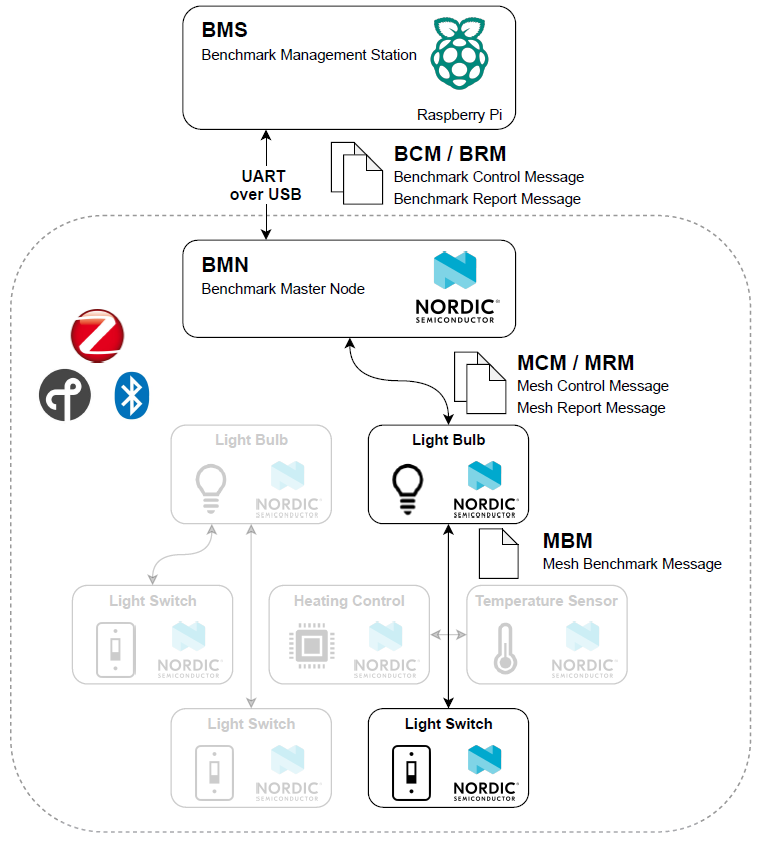
\includegraphics[width=0.7\textwidth]{Mesh_Testkonzept.png}
	\caption{Konzeptschema für den Ablauf eines Mesh Benchmarks.}\label{fig:MeshTestKonzept}
\end{figure}


%\subsubsection{Nodes}\label{subsubsec:Nodes}

\subsubsection{Messages}\label{subsubsec:Messages}
In der Abbildung \ref{fig:MeshTestKonzept} sind verschiedene Messages dargestellt. Dabei handelt es sich um die Nachrichten die zwischen den einzelnen Teilen des Testaufbaus versendet werden und schliesslich einen Benchmark ausmachen. Die Messages besitzen Funktionen:

\paragraph{Mesh Benchmark Message (MBM)}
Die MBM ist jene Message welche die eigentlichen Messdaten produziert und diese sogleich unter den BSN (Mesh Knoten) überträgt. Anhand dieser Messages werden die Parameter gemäss der Messwerttabelle in Anhang \ref{app:MesswerteBenchmarkMeshNetzwerke} erfasst. Bei den MBM handelt es sich also eigentlich um eine Sammlung von Messages welche je nach gewünschtem Messwert in Form und Anzahl unterschiedlich ausfallen können.

\paragraph{Mesh Control Message (MCM)}
Die MCM beinhaltet die Parameter für die Benchmarks welche vom BMN an alle BSN übertragen werden. Ausserdem werden damit Kontrollbefehle für die Benchmarks wie beispielsweise \textit{Start/Stop} sowie \textit{Laufzeit, Wiederholrate usw.} übertragen.

\paragraph{Mesh Report Message (MRM)}
Die MRM ist jene Message welche die Messwerte von den BSN an den BMN übertragen. Gleichzeitig wird damit auch gleich signalisiert, dass die Messung abgeschlossen wurde und mögliche Fehler oder sonstige Stati übermittelt.

\paragraph{Benchmark Control Message (BCM)}
Die BCM beschreibt die Nachrichten welche zur Steuerung eines Benchmarks von der BMS her dienen. Dabei handelt es sich um Befehle wie beispielsweise \textit{Start/Stop}. Die BCM werden via serieller USB-UART Schnittstelle von der BMS zum BMN übertragen.

\paragraph{Benchmark Report Message (BRM)}
Die BRM beschreiben Nachrichten welche den Status oder die Ergebnisse eines Benchmarks aus dem Mesh zurück an die BMS melden. Sie werden vom BMN initiiert und gelangen über eine die selbe USB-UART Schnittstelle wie die BCM zum BMS. Die BRM wird erst nach Abschluss des Benchmarks initiiert. Zuvor werden die Messdaten auf dem BMN zwischen gespeichert.



\subsection{Testszenarien}\label{subsec:TestszenarienMesh}
\todo[inline]{Testumgebungen sowie die Beziehungen der Knoten innerhalb der Mesh Netze beschreiben.}

Die Benchmarks der Mesh Protokolle sollen mit unterschiedlichen Bedingungen getestet werden wobei grundsätzlich eine reelle Anwendung nachgebaut werden soll. Zum einen gibt es unterschiedliche Beziehungen innerhalb des Mesh Netzwerks, zum anderen werden Testumgebungen unterschieden.

\subsection{Mesh Beziehungen}\label{subsec:MeshBeziehungen}

Innerhalb eines Mesh Netzwerks können 4 Beziehungen zwischen den Nodes für die Benchmarks unterschieden werden. Üblicherweise kommen mehrere oder sogar alle 4 Beziehungen innerhalb eines Netzwerkes gleichzeitig zum Einsatz. Abbildung \ref{fig:MeshTestBeziehungen} zeigt die Beziehungen.

\begin{itemize}
 	\item \textcolor{red}{Rot stellt eine einfache P2P Verbindung ohne Hop dar. Beispielweise schaltet ein einzelner Schalter eine einzelne, definierte Lichtquelle}
 	\item \textcolor{orange}{Orange ist eine many-to-one Verbindung in welcher mehrere Lichtschalter die selbe Lichtquelle schalten.}
 	\item \textcolor{cyan}{In blau ist eine klassiche one-to-many Topologie dargestellt in welcher beispielsweise ein Schalter mehrere Lichtquellen bedient.}
 	 \item \textcolor{green}{Grün dargestellt ist eine indirekte P2P Verbindung mit. Das bedeutet, dass Schalter und Lichtquelle keine direkte Verbindung zueinander haben und daher Mesh-typisch via einem oder mehreren Hops kommuniziert.}
\end{itemize}


\begin{figure}[H]
	\centering
	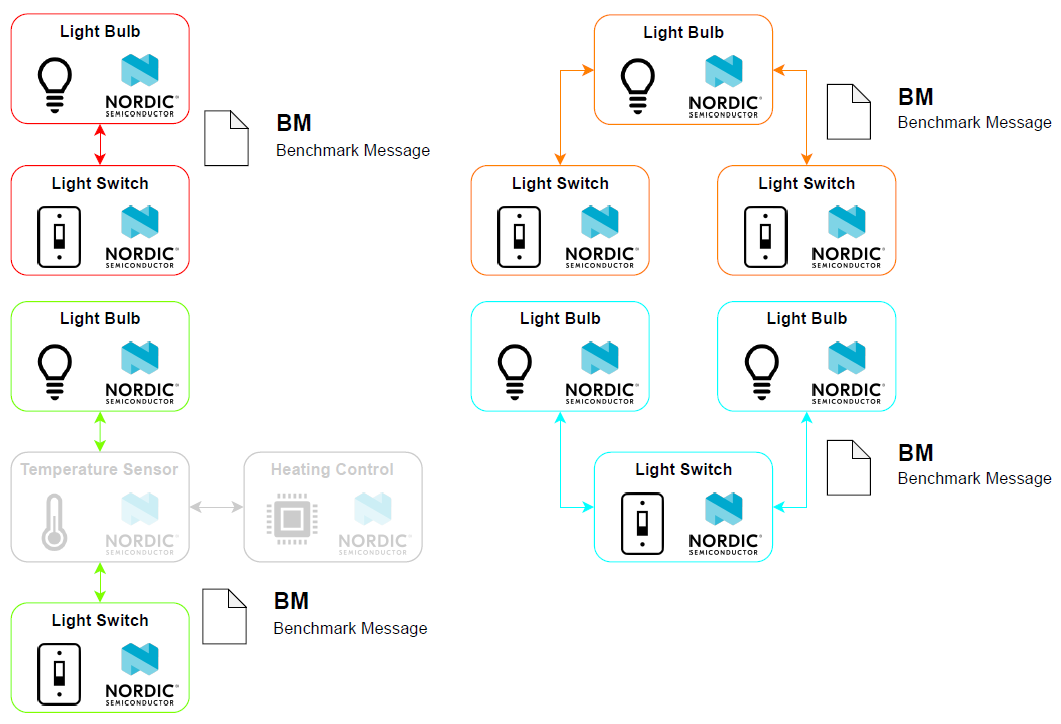
\includegraphics[width=1.0\textwidth]{Mesh_Test_Beziehungen.png}
	\caption{Beziehungen zwischen den Mesh Nodes innerhalb eines Benchmarks.}\label{fig:MeshTestBeziehungen}
\end{figure}


\subsection{Testumgebungen}\label{subsec:Testumgebungen}

Unterschiedliche Testumgebungen sollen die Benchmarks und schlussendlich den Vergleich der 3 Mesh Protokolle aussagekräftiger machen. Abbildung \ref{fig:MeshNetzwerkTestumgebungen} zeigt 5 unterschiedliche Umgebungen in denen Messungen durchgeführt werden sollen.

\begin{figure}[H]
	\centering
	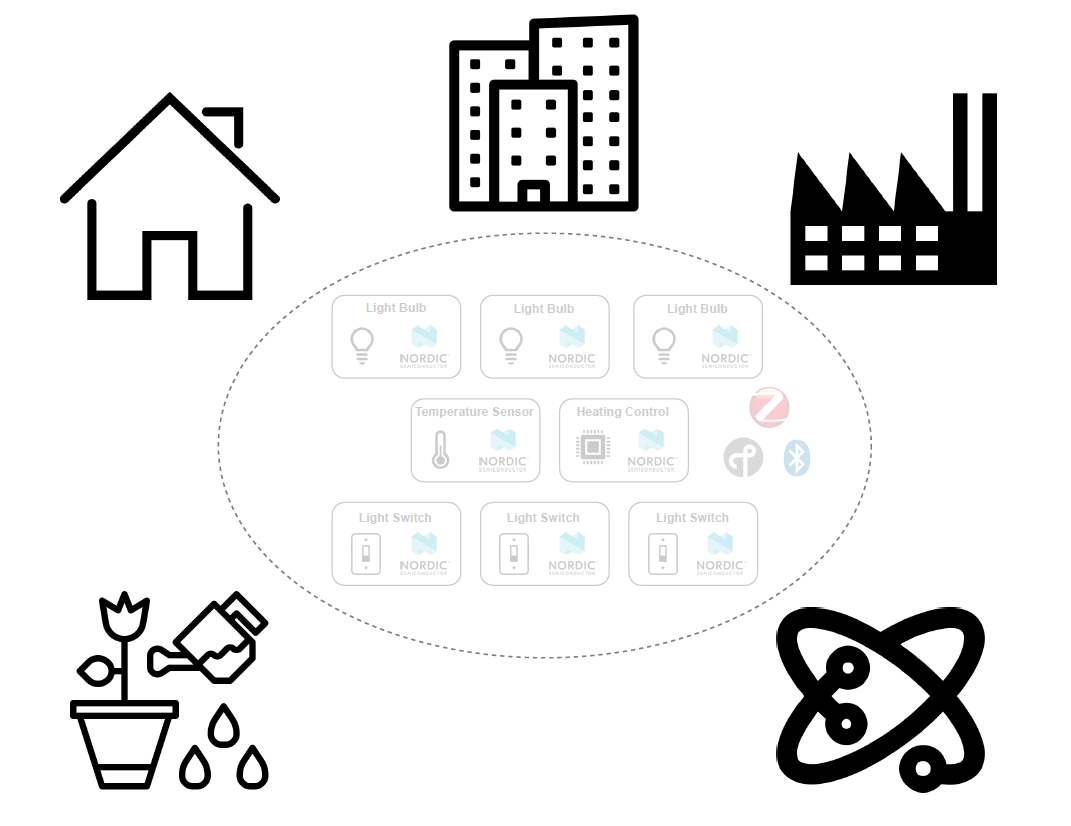
\includegraphics[width=1.0\textwidth]{Mesh_Testumgebung.png}
	\caption{Mesh Netzwerk Testumgebungen}\label{fig:MeshNetzwerkTestumgebungen}
\end{figure}

\todo[inline]{Bild anpassen.}

\paragraph{Haus}
Die Testgeräte werden in einem Einfamilienhaus installiert und repräsentieren damit eine flächendeckende Heim-Automatisierung.
	\begin{itemize}
		\item Einfamilienhaus über mehrere Etagen.
		\item Anzahl Sensoren und Aktoren vergleichbar gross.
		\item Node-Dichte relativ gering.
		\item Keine Beeinflussung durch Nachbarsysteme zu erwarten
	\end{itemize}
	
\paragraph{Wohnung}
Ebenfalls als Heim-Automatisierung gedacht werden die Messungen in einer Wohnung durchgeführt.
	\begin{itemize}
		\item Wohnung über eine Etage in einem Mehrfamilienhaus
		\item Anzahl Sensoren und Aktoren vergleichbar gross.
		\item Node-Dichte höher als im Haus.
		\item Mögliche Störeinflüsse durch andere Systeme von Nachbarn zu 					erwarten.
	\end{itemize}
	
\paragraph{Industrie}
Um eine Industrielle Anwendung zu vergleichen erfolgt eine Messung in einem Industriebetrieb.
	\begin{itemize}
		\item Industriebetrieb mit grosser Fläche.
		\item Grosse Anzahl Sensoren zur Überwachung von Produktionsprozessen. 				Vereinzelt Aktoren zur Ansteuerung von Anlageteilen.
		\item Hohe Node-Dichte.
		\item Mögliche Störeinflüsse durch Maschinen oder Abschirmwirkung durch 			metallische Gegenstände zu erwarten.
	\end{itemize}

\paragraph{Labor}
Der Laboraufbau ist ein Extremtest welcher die Leistungsgrenzen der Protokollstacks ausloten soll.
	\begin{itemize}
		\item Testaufbau unter Laborbedingungen auf engstem Raum.
		\item Ausgeglichene Anzahl Sensoren und Aktoren.
		\item Sehr Hohe Node-Dichte.
		\item Geringe bis keine Störbeeinflussung durch die Umgebung zu erwarten.
	\end{itemize}
	
\paragraph{Landwirtschaft (optional)}
Für die Überwachung und Kontrolle von landwirtschaftlichen Flächen kann ein Test auf offenem Feld erfolgen.
	\begin{itemize}
		\item Landwirtschaftsfläche mit grosser Ausbreitung (z.B. Gemüseanbau).
		\item Grosse Anzahl Sensoren. Nur wenige bis gar keine Aktoren.
		\item Sehr geringe Node-Dichte mit weiten Distanzen.
		\item Geringe bis keine Störbeeinflussung durch die Umgebung zu erwarten.
	\end{itemize}


\subsection{Ablauf}\label{subsec:AblaufMesh}
\todo[inline]{Ablauf eines Mesh Benchmarks aus Anwendersicht beschreiben.}

Ein Mesh Benchmark folgt einem klar definierten Ablauf. Die Abbildung \ref{fig:MeshTestKonzept} zeigt das Testkonzept in welchem auch der Ablauf eines Benchmarks bereits angedeutet ist.

\begin{enumerate}
	\item \textbf{Benchmark User-Init:}\\
	Auf dem Webinterface des BMS werden die gewünschten Parameter definiert und der Benchmark durch den Benutzer gestartet.
	\item \textbf{Benchmark Init BMN:}\\
	Die Parameter werden an den BMN übergeben welcher diese wiederum an alle teilnehmenden BSN weiterleitet. Mit einem Startsignal vom BMN wird der Benchmark auf den BSN gestartet.
	\item \textbf{Benchmark Prozess:}\\
	Die BSN führen den Benchmark Prozess mit den definierten Parametern aus. Dies geschieht autonom und jeweils nur zwischen den entsprechenden BSN die in einer direkten Beziehung zueinander stehen (siehe Mesh Beziehungen \ref{subsec:MeshBeziehungen}). Die entstehenden Messdaten werden auf den BSN zwischen gespeichert.
	\item \textbf{Reporting:}\\
	Nach Ablauf der Benchmark Zeit werden die Messdaten an den BMN übertragen. Dies erfolgt gesteuert durch den BMN welcher die Daten bei einem BSN nach dem anderen abfragt und direkt an das BMS weiterleitet.
	\item \textbf{Finish:}\\
	Der BMN kontrolliert ob er die Daten von sämtlichen BSN korrekt auslesen konnte und bestätigt das Ende der Messung gegenüber dem BMS.
	\item \textbf{Auswertung:}\\
	Das BMS beendet den Benchmark Vorgang, speichert die Messdaten in seiner Datenbank ab und bereitet diese grafisch auf. 
\end{enumerate}

\subsection{Messaufbau}\label{subsec:Messaufbau}
\todo[inline]{Wenn möglich Schema mit dem Aufbau der Messumgebung. Beschreibung der unterschiedlichen Standorte.}

\subsection{Messgrössen}\label{subsec:MessgrössenMesh}
\todo[inline]{Erläuterung der Messgrössen die erfasst werden sollen. Inkl. Beschreibung wie dies technisch umgesetzt wird.}

\subsection{Messreihe}\label{subsec:Messreihe}


\begin{table}[h]
\centering
\begin{tabular}{lccc} 
\toprule
 & BT Mesh & Thread & Zigbee \\ 
\hline
Benchmark Duration & 600s & 600s & 600s \\
Group addressing mode & Broadcast & Multicast & Directional \\
Message Ack (Appl. Layer) & No & No & No \\
Mesh Node Cnt. & 50 & 50 & 50 \\
Payload Size Small (Byte) & 8 & 8 & 8 \\
Payload Size Large (Byte) & 32 & 50 & 50 \\
\bottomrule
\end{tabular}
\caption{Allgemeine Benchmark Parameter}
\label{tab:AllgemeineBenchmarkParameter}
\end{table}
\todo[inline]{Wieso 32 und 50 Byte Unterschied erläutern}

\begin{table}[h]
\centering
\begin{tabular}{|c|c|c|c|c|c|} 
\cline{2-6}
\multicolumn{1}{c|}{} & \multicolumn{5}{c|}{Benchmark Parameter} \\ 
\hline
\textbf{Index}  & \textbf{Msg. Gen.}  & \textbf{Msg. Cnt.}  & \textbf{Payload }  & \textbf{Disturbance}  & \textbf{Msg. Density}  \\ 
\hline
1 & Seq. & 60 & Small & No & 0.1 \\ 
\hline
2 & Rand. & 60 & Small & No & 0.1 \\ 
\hline
3 & Seq. & 60 & Large & No & 0.1 \\ 
\hline
4 & Rand. & 60 & Large & No & 0.1 \\ 
\hline
5 & Rand. & 600 & Small & No & 1 \\ 
\hline
6 & Seq. & 60 & Small & Yes & 0.1 \\
\hline
\end{tabular}
\caption{Parameter Benchmark Messreihe}
\label{tab:ParameterBenchmarkMessreihe}
\end{table}



\begin{table}[h]
\centering
\begin{tabular}{lll} 
\toprule
Parameter: & Gültige Werte: & Bedeutung: \\ 
\hline
Msg. Gen & Seq./Rand. & Nachrichten Generierung sequentiell oder pseudozufällig. \\
Msg. Count & Ganze Zahlen & \begin{tabular}[t]{@{}l@{}}Anzahl der Nachrichten die pro Client Node\\versendet werden. \end{tabular} \\
Payload & Small/Large & \begin{tabular}[t]{@{}l@{}}Grosse oder Kleine Payload gemäss Definition\\in Tabelle \ref{tab:AllgemeineBenchmarkParameter}.~\end{tabular} \\
Disturbance & Yes/No & \begin{tabular}[t]{@{}l@{}}Gewollte Störung durch P2P Testinfrastruktur auf\\dem selben Channel. \end{tabular} \\
Msg. Density & - & \begin{tabular}[t]{@{}l@{}}Dichte der Nachrichten. Verhältnis zwischen\\Benchmark Duration und Msg. Count. \end{tabular} \\
\bottomrule
\end{tabular}
\caption{Bedeutung Benchmark Parameter}
\label{tab:BedeutungBenchmarkParameter}
\end{table}


\subsection{Messdatenerfassung und Auswertung}\label{subsec:MessdatenerfassungundAuswertung}
\todo[inline]{Beschreibung der Hard und Software für die Datenerfassung und die Auswertung.}

\subsection{Messerwartung}\label{subsec:Messerwartung}
\todo[inline]{Welche Resultate werden erwartet. Welcher der drei Stacks ist vermeintlich der Beste?}

